\documentclass[twoside]{book}

% Packages required by doxygen
\usepackage{fixltx2e}
\usepackage{calc}
\usepackage{doxygen}
\usepackage[export]{adjustbox} % also loads graphicx
\usepackage{graphicx}
\usepackage[utf8]{inputenc}
\usepackage{makeidx}
\usepackage{multicol}
\usepackage{multirow}
\PassOptionsToPackage{warn}{textcomp}
\usepackage{textcomp}
\usepackage[nointegrals]{wasysym}
\usepackage[table]{xcolor}

% Font selection
\usepackage[T1]{fontenc}
\usepackage[scaled=.90]{helvet}
\usepackage{courier}
\usepackage{amssymb}
\usepackage{sectsty}
\renewcommand{\familydefault}{\sfdefault}
\allsectionsfont{%
  \fontseries{bc}\selectfont%
  \color{darkgray}%
}
\renewcommand{\DoxyLabelFont}{%
  \fontseries{bc}\selectfont%
  \color{darkgray}%
}
\newcommand{\+}{\discretionary{\mbox{\scriptsize$\hookleftarrow$}}{}{}}

% Page & text layout
\usepackage{geometry}
\geometry{%
  a4paper,%
  top=2.5cm,%
  bottom=2.5cm,%
  left=2.5cm,%
  right=2.5cm%
}
\tolerance=750
\hfuzz=15pt
\hbadness=750
\setlength{\emergencystretch}{15pt}
\setlength{\parindent}{0cm}
\setlength{\parskip}{3ex plus 2ex minus 2ex}
\makeatletter
\renewcommand{\paragraph}{%
  \@startsection{paragraph}{4}{0ex}{-1.0ex}{1.0ex}{%
    \normalfont\normalsize\bfseries\SS@parafont%
  }%
}
\renewcommand{\subparagraph}{%
  \@startsection{subparagraph}{5}{0ex}{-1.0ex}{1.0ex}{%
    \normalfont\normalsize\bfseries\SS@subparafont%
  }%
}
\makeatother

% Headers & footers
\usepackage{fancyhdr}
\pagestyle{fancyplain}
\fancyhead[LE]{\fancyplain{}{\bfseries\thepage}}
\fancyhead[CE]{\fancyplain{}{}}
\fancyhead[RE]{\fancyplain{}{\bfseries\leftmark}}
\fancyhead[LO]{\fancyplain{}{\bfseries\rightmark}}
\fancyhead[CO]{\fancyplain{}{}}
\fancyhead[RO]{\fancyplain{}{\bfseries\thepage}}
\fancyfoot[LE]{\fancyplain{}{}}
\fancyfoot[CE]{\fancyplain{}{}}
\fancyfoot[RE]{\fancyplain{}{\bfseries\scriptsize Generated by Doxygen }}
\fancyfoot[LO]{\fancyplain{}{\bfseries\scriptsize Generated by Doxygen }}
\fancyfoot[CO]{\fancyplain{}{}}
\fancyfoot[RO]{\fancyplain{}{}}
\renewcommand{\footrulewidth}{0.4pt}
\renewcommand{\chaptermark}[1]{%
  \markboth{#1}{}%
}
\renewcommand{\sectionmark}[1]{%
  \markright{\thesection\ #1}%
}

% Indices & bibliography
\usepackage{natbib}
\usepackage[titles]{tocloft}
\setcounter{tocdepth}{3}
\setcounter{secnumdepth}{5}
\makeindex

% Hyperlinks (required, but should be loaded last)
\usepackage{ifpdf}
\ifpdf
  \usepackage[pdftex,pagebackref=true]{hyperref}
\else
  \usepackage[ps2pdf,pagebackref=true]{hyperref}
\fi
\hypersetup{%
  colorlinks=true,%
  linkcolor=blue,%
  citecolor=blue,%
  unicode%
}

% Custom commands
\newcommand{\clearemptydoublepage}{%
  \newpage{\pagestyle{empty}\cleardoublepage}%
}

\usepackage{caption}
\captionsetup{labelsep=space,justification=centering,font={bf},singlelinecheck=off,skip=4pt,position=top}

%===== C O N T E N T S =====

\begin{document}

% Titlepage & ToC
\hypersetup{pageanchor=false,
             bookmarksnumbered=true,
             pdfencoding=unicode
            }
\pagenumbering{alph}
\begin{titlepage}
\vspace*{7cm}
\begin{center}%
{\Large My Project }\\
\vspace*{1cm}
{\large Generated by Doxygen 1.8.12}\\
\end{center}
\end{titlepage}
\clearemptydoublepage
\pagenumbering{roman}
\tableofcontents
\clearemptydoublepage
\pagenumbering{arabic}
\hypersetup{pageanchor=true}

%--- Begin generated contents ---
\chapter{Hierarchical Index}
\section{Class Hierarchy}
This inheritance list is sorted roughly, but not completely, alphabetically\+:\begin{DoxyCompactList}
\item \contentsline{section}{Base\+Device}{\pageref{class_base_device}}{}
\item Q\+Dialog\begin{DoxyCompactList}
\item \contentsline{section}{Ip\+Dialog}{\pageref{class_ip_dialog}}{}
\end{DoxyCompactList}
\item \contentsline{section}{Ui\+\_\+\+Ip\+Dialog}{\pageref{class_ui___ip_dialog}}{}
\begin{DoxyCompactList}
\item \contentsline{section}{Ui\+:\+:Ip\+Dialog}{\pageref{class_ui_1_1_ip_dialog}}{}
\end{DoxyCompactList}
\end{DoxyCompactList}

\chapter{Class Index}
\section{Class List}
Here are the classes, structs, unions and interfaces with brief descriptions\+:\begin{DoxyCompactList}
\item\contentsline{section}{\hyperlink{class_base_device}{Base\+Device} \\*Базовый класс связки с приборами через библиотеку visa }{\pageref{class_base_device}}{}
\item\contentsline{section}{\hyperlink{class_ip_dialog}{Ip\+Dialog} }{\pageref{class_ip_dialog}}{}
\item\contentsline{section}{\hyperlink{class_ui_1_1_ip_dialog}{Ui\+::\+Ip\+Dialog} }{\pageref{class_ui_1_1_ip_dialog}}{}
\item\contentsline{section}{\hyperlink{class_ui___ip_dialog}{Ui\+\_\+\+Ip\+Dialog} }{\pageref{class_ui___ip_dialog}}{}
\end{DoxyCompactList}

\chapter{Class Documentation}
\hypertarget{class_base_device}{}\section{Base\+Device Class Reference}
\label{class_base_device}\index{Base\+Device@{Base\+Device}}


Базовый класс связки с приборами через библиотеку visa.  




{\ttfamily \#include $<$basedevice.\+h$>$}

\subsection*{Public Member Functions}
\begin{DoxyCompactItemize}
\item 
\hyperlink{class_base_device_a163a3af4b53ebe0a947c62074f6216f3}{Base\+Device} ()
\begin{DoxyCompactList}\small\item\em Конструктор. \end{DoxyCompactList}\item 
Q\+String \hyperlink{class_base_device_ae1cd92f757a47b0a7ebc0dfa2247e313}{Connect\+Device} (Q\+String type\+Connect, Q\+String type\+Adder)
\begin{DoxyCompactList}\small\item\em Метод для состыковки с прибором \end{DoxyCompactList}\item 
Q\+String \hyperlink{class_base_device_af6b2ad4cb09e0d0115f0e883e747bf9b}{Disconnect\+Device} ()
\begin{DoxyCompactList}\small\item\em Метод для рассоединения с прибором \end{DoxyCompactList}\item 
\hypertarget{class_base_device_afeaaa2f48222274407eb7c23194b181f}{}\label{class_base_device_afeaaa2f48222274407eb7c23194b181f} 
Q\+String \hyperlink{class_base_device_afeaaa2f48222274407eb7c23194b181f}{I\+DN} ()
\begin{DoxyCompactList}\small\item\em Базовые функции. Возвращают Q\+String. Ежели строка пустая-\/ Успешное выполнение команды, нет-\/ читаем. \end{DoxyCompactList}\item 
\hypertarget{class_base_device_acfb9d32117cf99db00c3098987e8f68e}{}\label{class_base_device_acfb9d32117cf99db00c3098987e8f68e} 
Q\+String {\bfseries R\+ST} ()
\item 
\hypertarget{class_base_device_aded8d300b85bf23b7343c0d609c0a906}{}\label{class_base_device_aded8d300b85bf23b7343c0d609c0a906} 
Q\+String {\bfseries T\+ST} ()
\item 
\hypertarget{class_base_device_a4be114e86b77b0fb111935fffb7fae96}{}\label{class_base_device_a4be114e86b77b0fb111935fffb7fae96} 
Q\+String {\bfseries W\+AI} ()
\end{DoxyCompactItemize}
\subsection*{Protected Member Functions}
\begin{DoxyCompactItemize}
\item 
Q\+String \hyperlink{class_base_device_a94fda8711eb27d0c9abbe470a30a32bf}{Error\+Function} (Vi\+Status status)
\begin{DoxyCompactList}\small\item\em Метод поиска описания ошибки. Ежели такой нет, то на выходе будет номер. \end{DoxyCompactList}\item 
Q\+String \hyperlink{class_base_device_a8e7de3e063defc28d0bd3d850099d4a5}{Write\+Command} (Q\+String command)
\begin{DoxyCompactList}\small\item\em Универсальная функция для записи в прибор. Использует vi\+Write. \end{DoxyCompactList}\item 
Q\+String \hyperlink{class_base_device_ac73856a92b58fd249e41bed55cee55ef}{Read\+Device} ()
\begin{DoxyCompactList}\small\item\em Универсальная функция для чтения из прибора. Использует vi\+Read. \end{DoxyCompactList}\end{DoxyCompactItemize}
\subsection*{Protected Attributes}
\begin{DoxyCompactItemize}
\item 
\hypertarget{class_base_device_a804561b100ae59ba8785ecdb23e14384}{}\label{class_base_device_a804561b100ae59ba8785ecdb23e14384} 
bool \hyperlink{class_base_device_a804561b100ae59ba8785ecdb23e14384}{flag\+\_\+connect}
\begin{DoxyCompactList}\small\item\em Флаг проверки подключения прибора \end{DoxyCompactList}\end{DoxyCompactItemize}


\subsection{Detailed Description}
Базовый класс связки с приборами через библиотеку visa. 

\begin{DoxyVersion}{Version}
1.\+0 
\end{DoxyVersion}
\begin{DoxyWarning}{Warning}
Данный класс создан только в учебных целях
\end{DoxyWarning}
Обычный базовый класс для работы с приборами. Все методы возвращают строку. Если ошибок нет -\/ нулевую строку. 

\subsection{Constructor \& Destructor Documentation}
\hypertarget{class_base_device_a163a3af4b53ebe0a947c62074f6216f3}{}\label{class_base_device_a163a3af4b53ebe0a947c62074f6216f3} 
\index{Base\+Device@{Base\+Device}!Base\+Device@{Base\+Device}}
\index{Base\+Device@{Base\+Device}!Base\+Device@{Base\+Device}}
\subsubsection{\texorpdfstring{Base\+Device()}{BaseDevice()}}
{\footnotesize\ttfamily Base\+Device\+::\+Base\+Device (\begin{DoxyParamCaption}{ }\end{DoxyParamCaption})}



Конструктор. 

Инициализация Error\+List значениями, очистка буфера, Visa параметров, отвечающих за подклчение к прибору. Установка флага flag\+\_\+connect.

У Андрея за запись/чтение строки, тип double, отвечает printf/scanf Чтение строки в виде буфера и массива vi\+Read. 

\subsection{Member Function Documentation}
\hypertarget{class_base_device_ae1cd92f757a47b0a7ebc0dfa2247e313}{}\label{class_base_device_ae1cd92f757a47b0a7ebc0dfa2247e313} 
\index{Base\+Device@{Base\+Device}!Connect\+Device@{Connect\+Device}}
\index{Connect\+Device@{Connect\+Device}!Base\+Device@{Base\+Device}}
\subsubsection{\texorpdfstring{Connect\+Device()}{ConnectDevice()}}
{\footnotesize\ttfamily Q\+String Base\+Device\+::\+Connect\+Device (\begin{DoxyParamCaption}\item[{Q\+String}]{type\+Connect,  }\item[{Q\+String}]{type\+Adder }\end{DoxyParamCaption})}



Метод для состыковки с прибором 


\begin{DoxyParams}[1]{Parameters}
\mbox{\tt in}  & {\em type\+Connect} & -\/ тип соединения\+: T\+C\+P\+IP \\
\hline
\mbox{\tt in}  & {\em type\+Adder} & -\/ адрес. Для T\+C\+P\+IP это\+: 192.\+168.\+70.\+39 \\
\hline
\end{DoxyParams}
\begin{DoxyReturn}{Returns}
Строку Q\+String. Ежели строка пустая-\/ Успешное выполнение команды, нет-\/ читаем. 
\end{DoxyReturn}
\hypertarget{class_base_device_af6b2ad4cb09e0d0115f0e883e747bf9b}{}\label{class_base_device_af6b2ad4cb09e0d0115f0e883e747bf9b} 
\index{Base\+Device@{Base\+Device}!Disconnect\+Device@{Disconnect\+Device}}
\index{Disconnect\+Device@{Disconnect\+Device}!Base\+Device@{Base\+Device}}
\subsubsection{\texorpdfstring{Disconnect\+Device()}{DisconnectDevice()}}
{\footnotesize\ttfamily Q\+String Base\+Device\+::\+Disconnect\+Device (\begin{DoxyParamCaption}{ }\end{DoxyParamCaption})}



Метод для рассоединения с прибором 

\begin{DoxyReturn}{Returns}
Строку Q\+String. Ежели строка пустая-\/ Успешное выполнение команды, нет-\/ читаем. 
\end{DoxyReturn}
\hypertarget{class_base_device_a94fda8711eb27d0c9abbe470a30a32bf}{}\label{class_base_device_a94fda8711eb27d0c9abbe470a30a32bf} 
\index{Base\+Device@{Base\+Device}!Error\+Function@{Error\+Function}}
\index{Error\+Function@{Error\+Function}!Base\+Device@{Base\+Device}}
\subsubsection{\texorpdfstring{Error\+Function()}{ErrorFunction()}}
{\footnotesize\ttfamily Q\+String Base\+Device\+::\+Error\+Function (\begin{DoxyParamCaption}\item[{Vi\+Status}]{status }\end{DoxyParamCaption})\hspace{0.3cm}{\ttfamily [protected]}}



Метод поиска описания ошибки. Ежели такой нет, то на выходе будет номер. 


\begin{DoxyParams}[1]{Parameters}
\mbox{\tt in}  & {\em status(переменная} & типа Vi\+Status) \\
\hline
\end{DoxyParams}
\begin{DoxyReturn}{Returns}
Строку Q\+String с номером ошибки. 
\end{DoxyReturn}
\hypertarget{class_base_device_ac73856a92b58fd249e41bed55cee55ef}{}\label{class_base_device_ac73856a92b58fd249e41bed55cee55ef} 
\index{Base\+Device@{Base\+Device}!Read\+Device@{Read\+Device}}
\index{Read\+Device@{Read\+Device}!Base\+Device@{Base\+Device}}
\subsubsection{\texorpdfstring{Read\+Device()}{ReadDevice()}}
{\footnotesize\ttfamily Q\+String Base\+Device\+::\+Read\+Device (\begin{DoxyParamCaption}{ }\end{DoxyParamCaption})\hspace{0.3cm}{\ttfamily [protected]}}



Универсальная функция для чтения из прибора. Использует vi\+Read. 

\begin{DoxyReturn}{Returns}
Строку Q\+String. Ежели строка пустая-\/ Успешное выполнение команды, нет-\/ читаем. 
\end{DoxyReturn}
\hypertarget{class_base_device_a8e7de3e063defc28d0bd3d850099d4a5}{}\label{class_base_device_a8e7de3e063defc28d0bd3d850099d4a5} 
\index{Base\+Device@{Base\+Device}!Write\+Command@{Write\+Command}}
\index{Write\+Command@{Write\+Command}!Base\+Device@{Base\+Device}}
\subsubsection{\texorpdfstring{Write\+Command()}{WriteCommand()}}
{\footnotesize\ttfamily Q\+String Base\+Device\+::\+Write\+Command (\begin{DoxyParamCaption}\item[{Q\+String}]{command }\end{DoxyParamCaption})\hspace{0.3cm}{\ttfamily [protected]}}



Универсальная функция для записи в прибор. Использует vi\+Write. 


\begin{DoxyParams}[1]{Parameters}
\mbox{\tt in}  & {\em command} & -\/ строковая команда, согласно документации на прибор \\
\hline
\end{DoxyParams}
\begin{DoxyReturn}{Returns}
Строку Q\+String. Ежели строка пустая-\/ Успешное выполнение команды, нет-\/ читаем. 
\end{DoxyReturn}


The documentation for this class was generated from the following files\+:\begin{DoxyCompactItemize}
\item 
basedevice.\+h\item 
basedevice.\+cpp\end{DoxyCompactItemize}

\hypertarget{class_ip_dialog}{}\section{Ip\+Dialog Class Reference}
\label{class_ip_dialog}\index{Ip\+Dialog@{Ip\+Dialog}}
Inheritance diagram for Ip\+Dialog\+:\begin{figure}[H]
\begin{center}
\leavevmode
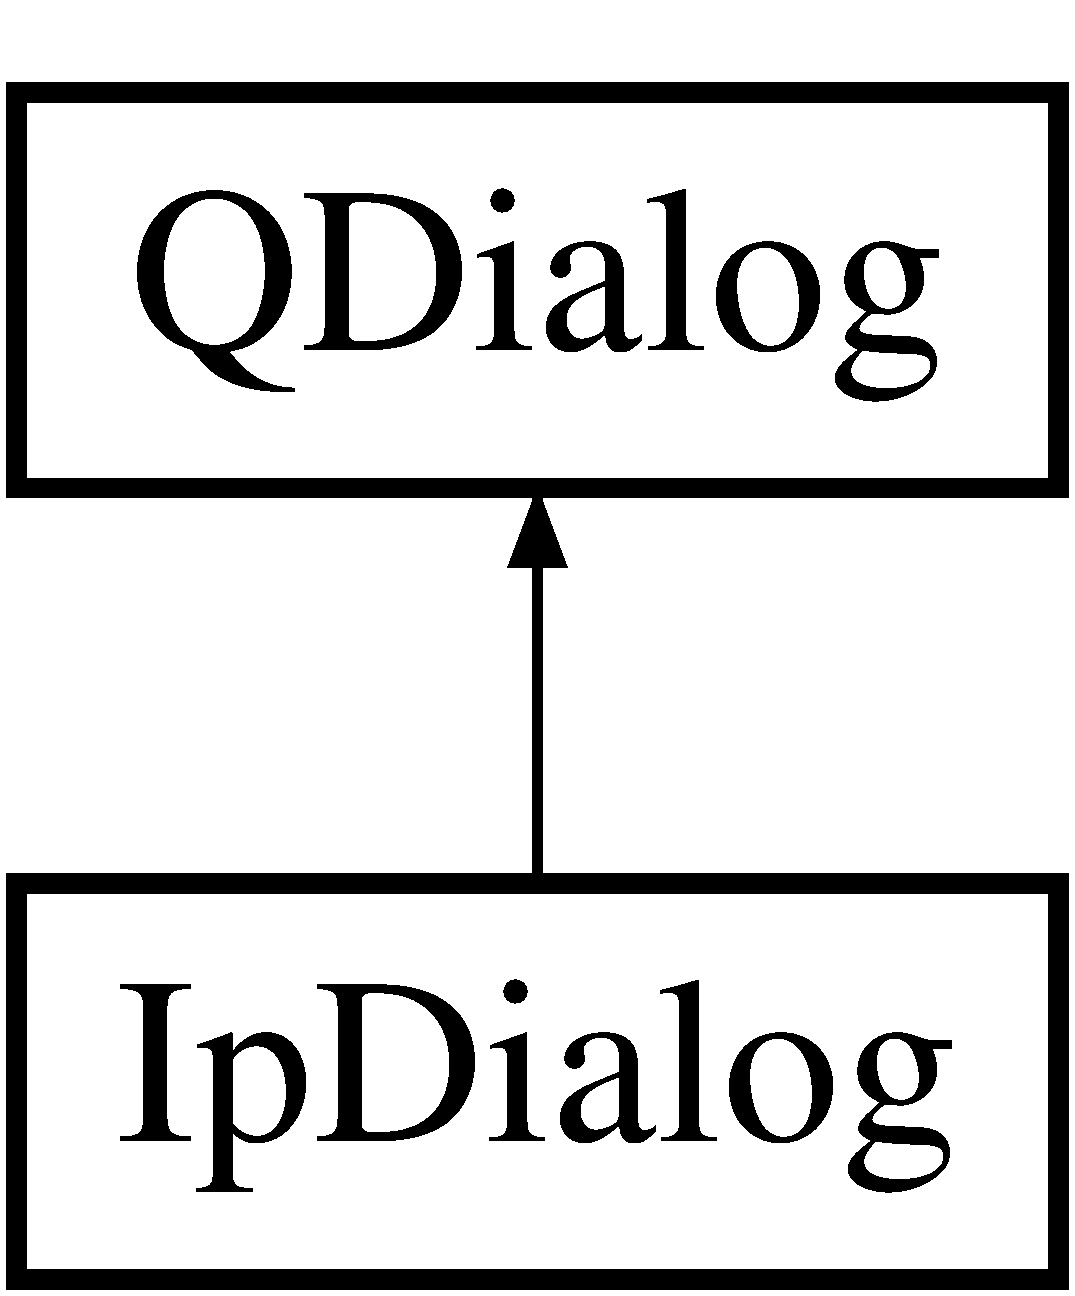
\includegraphics[height=2.000000cm]{class_ip_dialog}
\end{center}
\end{figure}
\subsection*{Public Member Functions}
\begin{DoxyCompactItemize}
\item 
\hypertarget{class_ip_dialog_a3508b87201acf6954baee640045fe505}{}\label{class_ip_dialog_a3508b87201acf6954baee640045fe505} 
{\bfseries Ip\+Dialog} (Q\+Widget $\ast$parent=0)
\end{DoxyCompactItemize}


The documentation for this class was generated from the following files\+:\begin{DoxyCompactItemize}
\item 
ipdialog.\+h\item 
ipdialog.\+cpp\end{DoxyCompactItemize}

\hypertarget{class_ui_1_1_ip_dialog}{}\section{Ui\+:\+:Ip\+Dialog Class Reference}
\label{class_ui_1_1_ip_dialog}\index{Ui\+::\+Ip\+Dialog@{Ui\+::\+Ip\+Dialog}}
Inheritance diagram for Ui\+:\+:Ip\+Dialog\+:\begin{figure}[H]
\begin{center}
\leavevmode
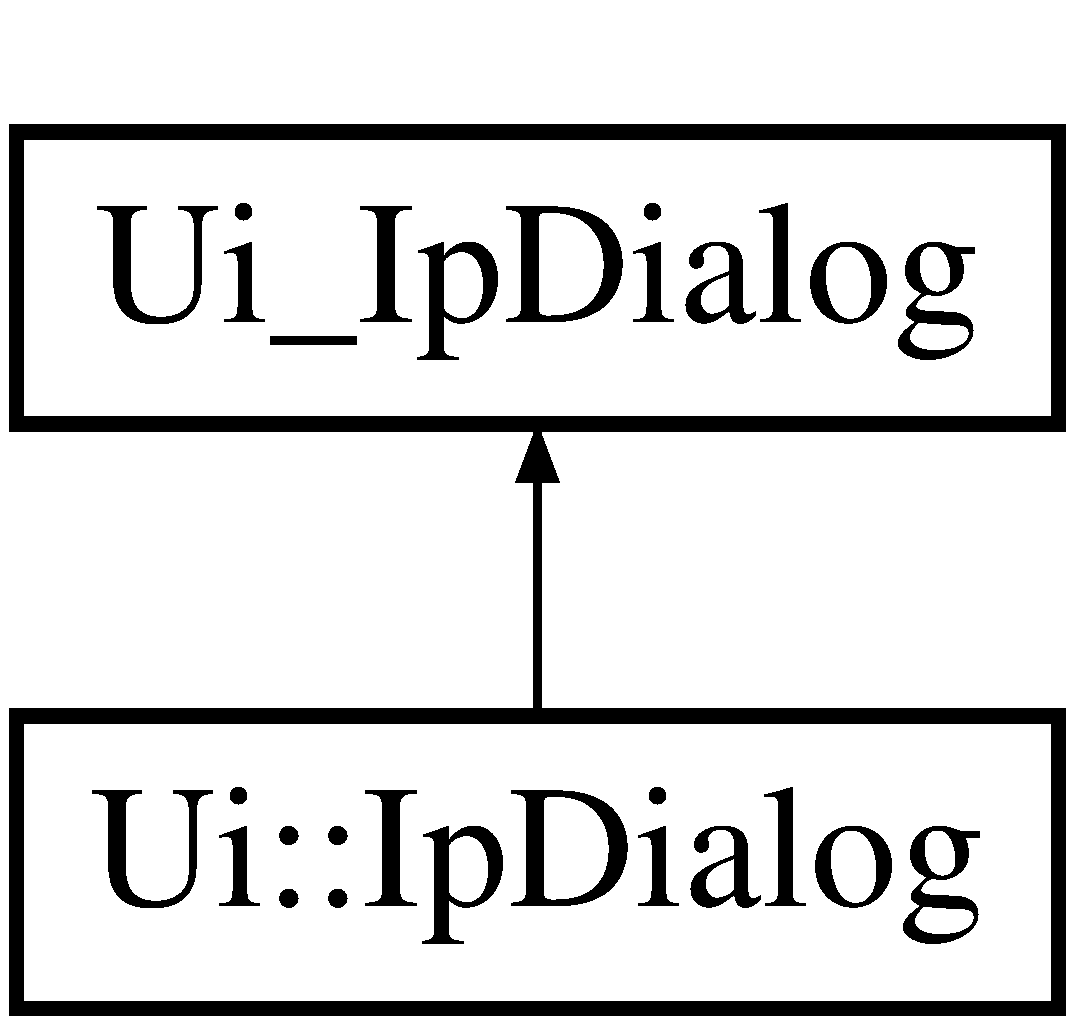
\includegraphics[height=2.000000cm]{class_ui_1_1_ip_dialog}
\end{center}
\end{figure}
\subsection*{Additional Inherited Members}


The documentation for this class was generated from the following file\+:\begin{DoxyCompactItemize}
\item 
ui\+\_\+ipdialog.\+h\end{DoxyCompactItemize}

\hypertarget{class_ui___ip_dialog}{}\section{Ui\+\_\+\+Ip\+Dialog Class Reference}
\label{class_ui___ip_dialog}\index{Ui\+\_\+\+Ip\+Dialog@{Ui\+\_\+\+Ip\+Dialog}}
Inheritance diagram for Ui\+\_\+\+Ip\+Dialog\+:\begin{figure}[H]
\begin{center}
\leavevmode
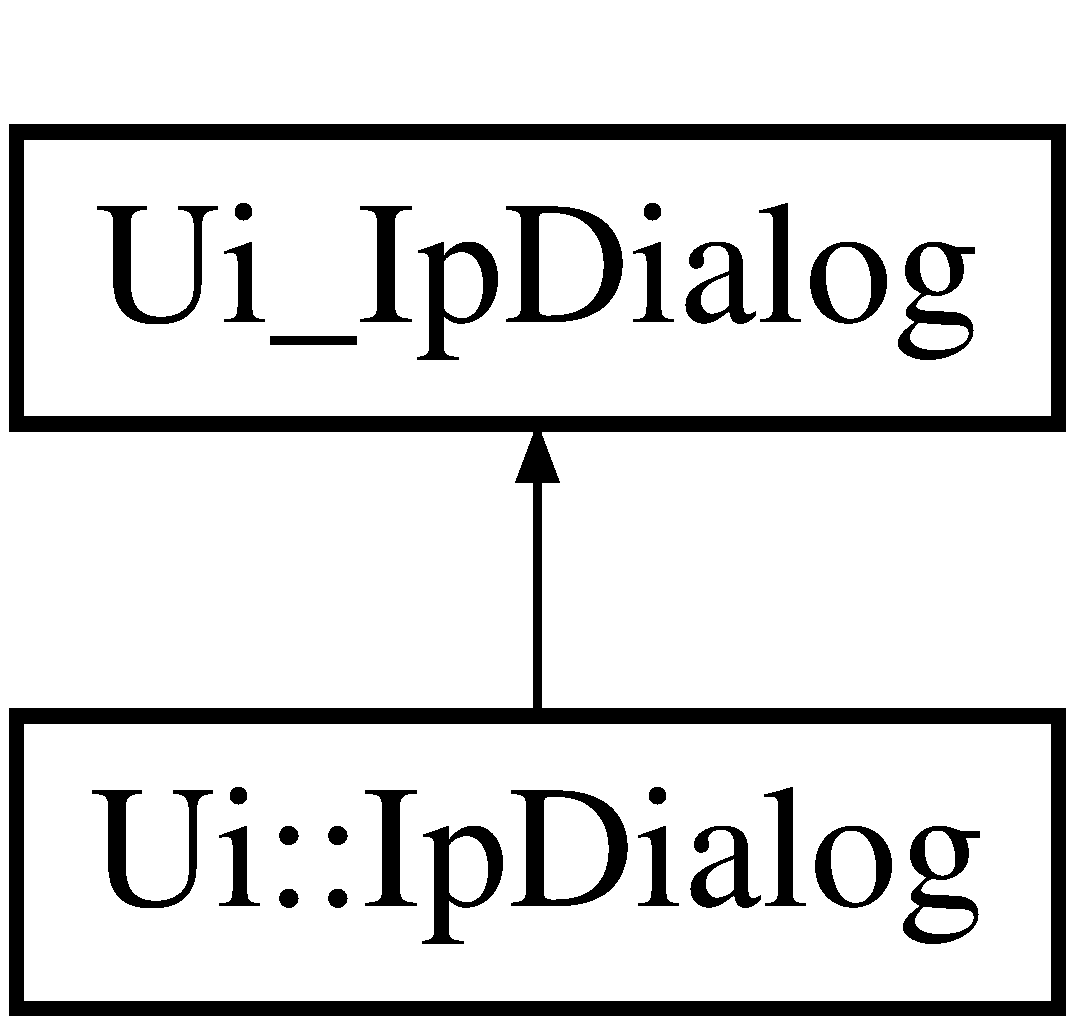
\includegraphics[height=2.000000cm]{class_ui___ip_dialog}
\end{center}
\end{figure}
\subsection*{Public Member Functions}
\begin{DoxyCompactItemize}
\item 
\hypertarget{class_ui___ip_dialog_a8fa6dd70ea0b48184c9d299ddc8c8897}{}\label{class_ui___ip_dialog_a8fa6dd70ea0b48184c9d299ddc8c8897} 
void {\bfseries setup\+Ui} (Q\+Dialog $\ast$\hyperlink{class_ip_dialog}{Ip\+Dialog})
\item 
\hypertarget{class_ui___ip_dialog_a72f26d70dbe8b16bf86d5bc47249ae3b}{}\label{class_ui___ip_dialog_a72f26d70dbe8b16bf86d5bc47249ae3b} 
void {\bfseries retranslate\+Ui} (Q\+Dialog $\ast$\hyperlink{class_ip_dialog}{Ip\+Dialog})
\end{DoxyCompactItemize}
\subsection*{Public Attributes}
\begin{DoxyCompactItemize}
\item 
\hypertarget{class_ui___ip_dialog_a6cef9b74bd3cbb89dac46cbb9425635b}{}\label{class_ui___ip_dialog_a6cef9b74bd3cbb89dac46cbb9425635b} 
Q\+Push\+Button $\ast$ {\bfseries push\+Button}
\item 
\hypertarget{class_ui___ip_dialog_af410b16fe28fac2e2cab9a7841ab606a}{}\label{class_ui___ip_dialog_af410b16fe28fac2e2cab9a7841ab606a} 
Q\+Line\+Edit $\ast$ {\bfseries line\+Edit}
\end{DoxyCompactItemize}


The documentation for this class was generated from the following file\+:\begin{DoxyCompactItemize}
\item 
ui\+\_\+ipdialog.\+h\end{DoxyCompactItemize}

%--- End generated contents ---

% Index
\backmatter
\newpage
\phantomsection
\clearemptydoublepage
\addcontentsline{toc}{chapter}{Index}
\printindex

\end{document}
